\addtocontents{toc}{\protect\contentsline{chapter}{}{}{}}

\chapter{Review-Dokumenation}
\label{chap:reviewDokumenation}

Während der Erstellung der Dokumentation wurde ein Review-Prozess etabliert, um die Konsistenz des Abschlussberichts sicherzustellen (\prettyref{fig:reviewDokumentation}).

Alle Abschnitte der Dokumentation wurden hierfür in eine Tabelle eingetragen und zum Review freigegeben. Die Projektmitarbeiter entschieden sich im Anschluss selbstständig für einen Abschnitt der Dokumentation und teilten dem Autor seine Hinweise mit. Abschließend überarbeitete der Autor seinen Abschnitt und markierte diesen entsprechend in der Tabelle.

\begin{figure}[h!]
	\centering
	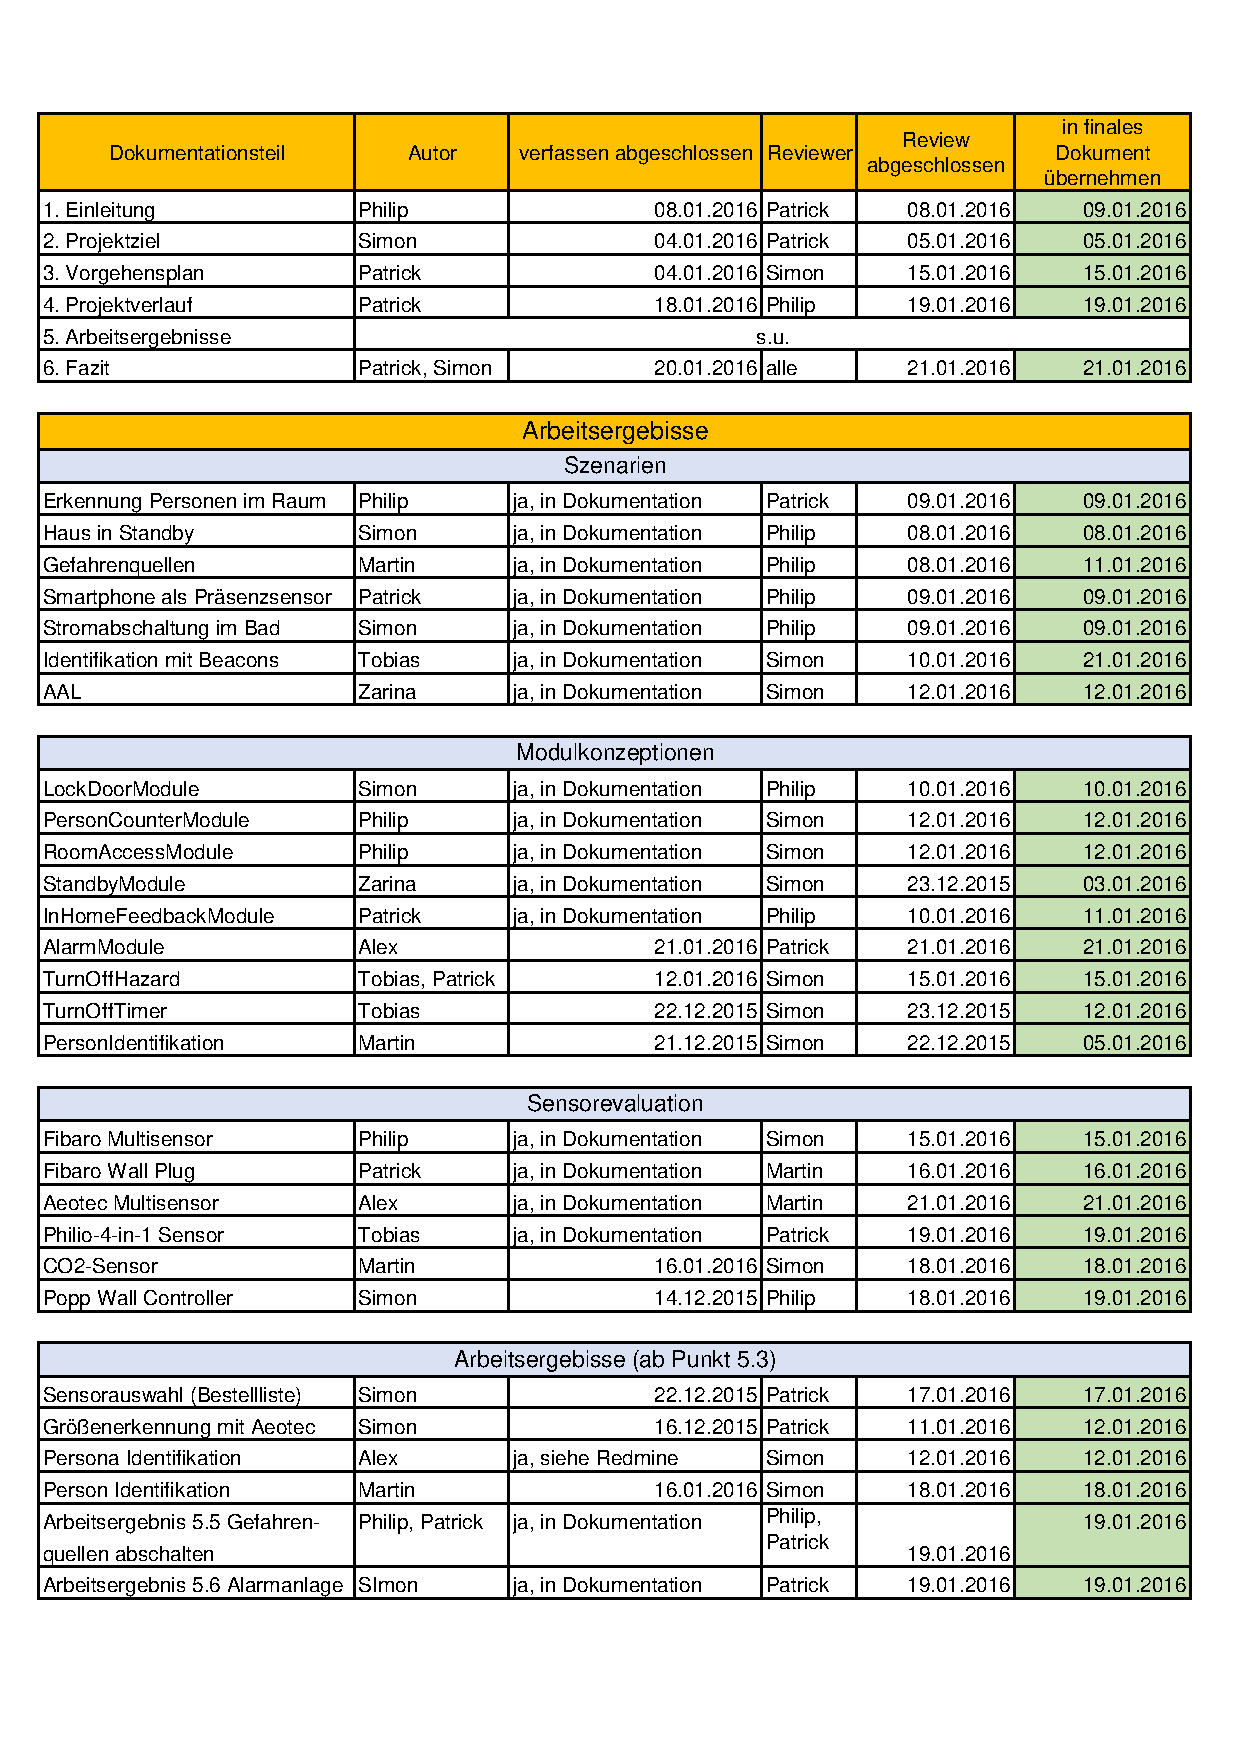
\includegraphics[width=1.0\textwidth]{img/Review-Dokumentation/Review-Dokumentation.pdf}
	\caption{Review-Dokumentation}
	\label{fig:reviewDokumentation}
\end{figure}